\documentclass[]{elsarticle} %review=doublespace preprint=single 5p=2 column
%%% Begin My package additions %%%%%%%%%%%%%%%%%%%
\usepackage[hyphens]{url}
\usepackage{lineno} % add
\providecommand{\tightlist}{%
  \setlength{\itemsep}{0pt}\setlength{\parskip}{0pt}}

\bibliographystyle{elsarticle-harv}
\biboptions{sort&compress} % For natbib
\usepackage{graphicx}
\usepackage{booktabs} % book-quality tables
%% Redefines the elsarticle footer
%\makeatletter
%\def\ps@pprintTitle{%
% \let\@oddhead\@empty
% \let\@evenhead\@empty
% \def\@oddfoot{\it \hfill\today}%
% \let\@evenfoot\@oddfoot}
%\makeatother

% A modified page layout
\textwidth 6.75in
\oddsidemargin -0.15in
\evensidemargin -0.15in
\textheight 9in
\topmargin -0.5in
%%%%%%%%%%%%%%%% end my additions to header

\usepackage[T1]{fontenc}
\usepackage{lmodern}
\usepackage{amssymb,amsmath}
\usepackage{ifxetex,ifluatex}
\usepackage{fixltx2e} % provides \textsubscript
% use upquote if available, for straight quotes in verbatim environments
\IfFileExists{upquote.sty}{\usepackage{upquote}}{}
\ifnum 0\ifxetex 1\fi\ifluatex 1\fi=0 % if pdftex
  \usepackage[utf8]{inputenc}
\else % if luatex or xelatex
  \usepackage{fontspec}
  \ifxetex
    \usepackage{xltxtra,xunicode}
  \fi
  \defaultfontfeatures{Mapping=tex-text,Scale=MatchLowercase}
  \newcommand{\euro}{€}
\fi
% use microtype if available
\IfFileExists{microtype.sty}{\usepackage{microtype}}{}
\usepackage{graphicx}
% We will generate all images so they have a width \maxwidth. This means
% that they will get their normal width if they fit onto the page, but
% are scaled down if they would overflow the margins.
\makeatletter
\def\maxwidth{\ifdim\Gin@nat@width>\linewidth\linewidth
\else\Gin@nat@width\fi}
\makeatother
\let\Oldincludegraphics\includegraphics
\renewcommand{\includegraphics}[1]{\Oldincludegraphics[width=\maxwidth]{#1}}
\ifxetex
  \usepackage[setpagesize=false, % page size defined by xetex
              unicode=false, % unicode breaks when used with xetex
              xetex]{hyperref}
\else
  \usepackage[unicode=true]{hyperref}
\fi
\hypersetup{breaklinks=true,
            bookmarks=true,
            pdfauthor={},
            pdftitle={Exploratory Network Analysis of Clinical Interactions in the ED},
            colorlinks=true,
            urlcolor=blue,
            linkcolor=magenta,
            pdfborder={0 0 0}}
\urlstyle{same}  % don't use monospace font for urls
\setlength{\parindent}{0pt}
\setlength{\parskip}{6pt plus 2pt minus 1pt}
\setlength{\emergencystretch}{3em}  % prevent overfull lines
\setcounter{secnumdepth}{0}
% Pandoc toggle for numbering sections (defaults to be off)
\setcounter{secnumdepth}{0}
% Pandoc header


\usepackage[nomarkers]{endfloat}

\begin{document}
\begin{frontmatter}

  \title{Exploratory Network Analysis of Clinical Interactions in the ED}
    \author[Emory University]{Tommy Flynn\corref{c1}}
   \ead{tjflynn@emory.edu} 
   \cortext[c1]{Corresponding Author}
      \address[Emory University]{Repository
(\url{https://github.com/tommyflynn/Flynn_N741_Project/tree/master/Flynn_Project})}
  
  \begin{abstract}
  Patient acuity in the Emergency Department is triaged at the beginning
  of the care process using the Emergency Severity Index (ESI) metric. The
  ESI is presumed to predict resource consumption in the ED, and is a
  validated predictor of hospital admission for the majority of ED
  patients. It is not sensitive to non-medical patient characteristics,
  such as patient race, nor is it accountable to changes in patient
  condition over time. ED administrators and charge nurses are left with
  an impression of the unit that does not reveal the reality of current
  paitient conditions or ED resources being utilized. The lack of
  real-time ED resource and patient condition information creates
  opportunities for unrecognized patient deterioration, medical errors,
  increased wait times, and decreased patient satisfaction. An objective
  measurement of patient resource consumption that passively observes and
  calulates relative patient need in real-time would allow charge nurses
  and administrators to make informed decisions for effective, efficient,
  and safe patient care. This study tests a novel approach to measuring
  patient acuity (ED resource consumption) using real-time location system
  (RTLS) contact data and network analysis. This paper presents the
  approach and analytic results of several ED contact networks in relation
  to patient acuity (ESI)
  \end{abstract}
  
 \end{frontmatter}

\section{Research Question \& Specific
Aims}\label{research-question-specific-aims}

\begin{itemize}
\tightlist
\item
  Can network analysis of clinical interactions between patients and
  staff provide insight into the complex Emergency Department patient
  care process? (Canto et al. 2000) Aim 1: Explore the network of
  clinical interactions in the ED between patients and staff to
  determine whether predictable patterns emerge in terms of centrality,
  density, and change over time. Aim 2: Test the assocaition between
  patient acuity and network position measure of eigenvector centrality
  of patient composite network, compared to the centrality of teh
  dynamic patient network (measure TBD).
\end{itemize}

\section{Background \& Objectives}\label{background-objectives}

Intelligent clinical monitoring software is not a new idea, but
advancements in the field of data science continue to yield powerful new
tools that may make such software a reality in the near future.(Yu et
al. 2015, Donoho (2017)) Real-time location systems (RTLS) are
increasingly common in hospitals across the nation, especially in
clinical areas where patient care and flow are both complex and
time-sensitive, such as the Emergency Department (ED).(Yao, Chu, and Li
2012) A bird's-eye view of a busy urban ED might resemble a hive of
frenzied bees, but as we have learned of beehives, patterns of work and
interactions within EDs are necessarily purposed and complexly adaptive
to the various needs of the system (or hive) as a whole.(Kridi,
Carvalho, and Gomes 2016) By leveraging the technology of RTLS and
analytical power of netowrk analysis, future ED monitoring systems will
provide ED leadership with real-time resource allocation and patient
condition information. The Emergency Severity Index (ESI) is a validated
metric used to triage patients in US Emergency Departments.(Tanabe et
al. 2004) That triage nurse may decide to involve the charge nurse or a
physician given various concerns about the patient. These interactions,
observed and measured by the Real Time Location System (RTLS), continue
as more patients are triaged, moved into patient rooms, and so on toward
a vast and complex network of interactions. This web of care is likely
to correlate with the amount and quality of care delivered to individual
patients. - \textbf{The purpose of this study is to explore the network
of clinical interactions that take place in the Emergency Department and
describe the raltionship between those network variables and patient
acuity.} To study this relationship, received permission to analyse
existing data that includes the following; the frequency and duration of
all face-to-face interactions (patients, providers, nurses, technicians,
\& administrators) that occured in the ED for 81 12hr shifts, the
location of those interactions, and individual patients' medical and
demographic characteristics including acuity, chief complaint, gender,
age, arrival mode, and disposition. The network structural
characteristics will be assessed in relation to the industry standard
acuity measure, the Emergency Severity Index (ESI), and potential
confounding variables. Using this data will require specific knowledge
of the R statistical packages, network analysis, and data science. See
Tables 1-4 for my learning goals with respective action items, timeline,
and outcomes.

\section{Methods}\label{methods}

\section{RTLS Data}\label{rtls-data}

This study applies a secondary data analysis design due to the
exploritory nature of the research aims. Data was made available with
permissions from the originating research team. The purpose of the
original study was to describe contact characteristics between patients
and staff in the ED of a busy urban hospital to inform cross-infection
control measures. Data were collected using a radio-frequency
identification system that triangulated patient and staff (nurses,
providers, and ancillary staff) locations within the ED at Emory
University Hospital Midtwon. Data for this secondary analysis were
collected using a prospective, longitudinal, observational design with a
random sampling of one day shift and one night shift per week for one
year, July 1, 2009 to June 30, 2010. This strategy was chosen to
minimize sampling bias related to seasonal or weekly fluctuations in
census, acuity, and ED staffing changes. Although a total of 104 shifts
were observed, the original research team retained only 81 shifts for
reasons related to issues with the RFID system and study staff sick
leave.(Lowery-North et al. 2013)
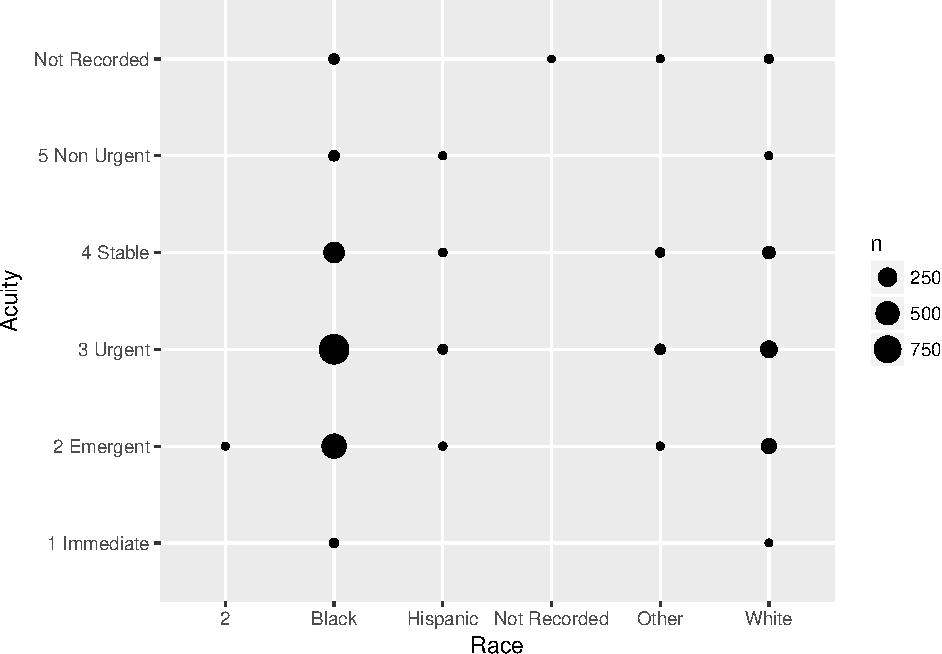
\includegraphics{Flynn_Project_files/figure-latex/assign datasets-1.pdf}
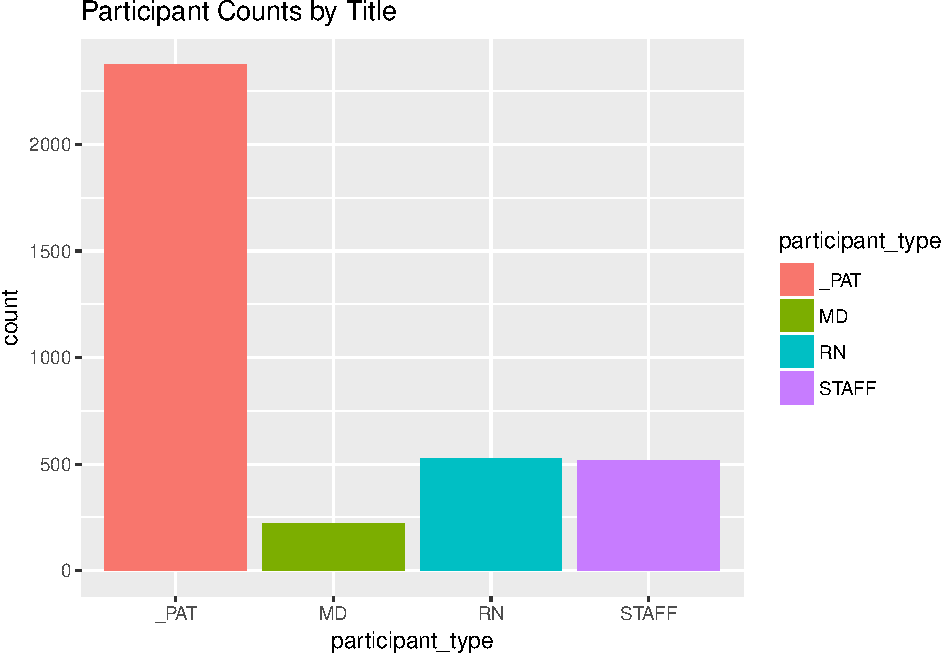
\includegraphics{Flynn_Project_files/figure-latex/assign datasets-2.pdf}

\begin{verbatim}
##  [1] "sid"                  "numshift"             "d8"                  
##  [4] "shift_ampm"           "Reason_shortShift"    "startd8time"         
##  [7] "endd8time"            "shift_d8_ampm"        "quarter"             
## [10] "weekday"              "H1N1"                 "ED_ARRIVAL"          
## [13] "ed_departure"         "durationInED"         "duration_UntilTag"   
## [16] "Sex"                  "Patient_Age_at_Visit" "Race"                
## [19] "Chief_Complaint"      "Acuity"               "Arr_Mode"            
## [22] "ED_Disposition"       "daysinED"             "MinutesInED"         
## [25] "AGE"                  "ILI_Syndrome"         "ILIwMissing"         
## [28] "hrsinED"              "timeCoveredbyShift"   "popnFreqbyshift"     
## [31] "shift_num_ampm"       "Participant_final"
\end{verbatim}

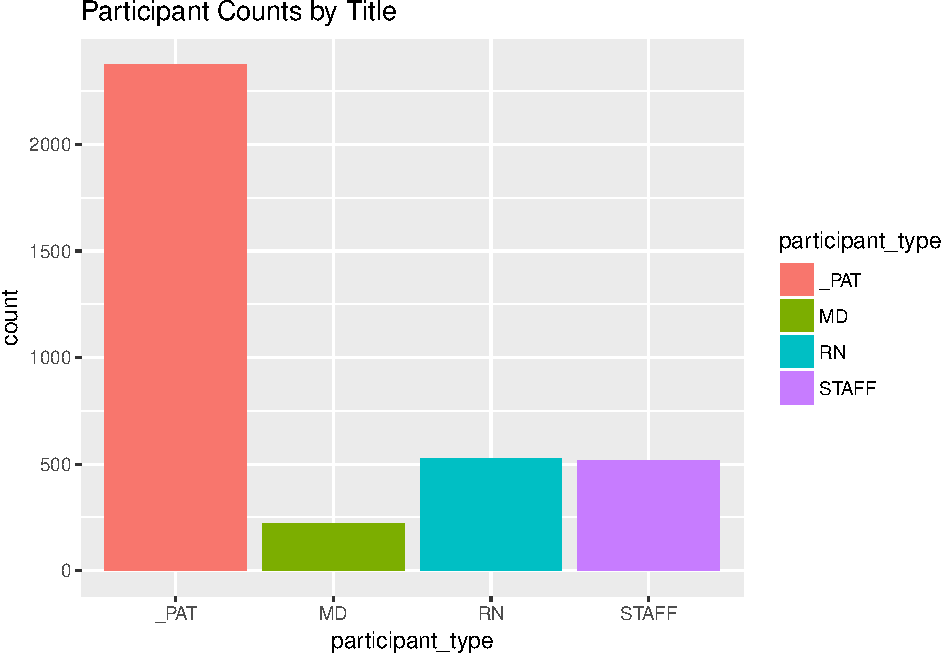
\includegraphics{Flynn_Project_files/figure-latex/assign datasets-3.pdf}
\#Results

\section{Analysis Plan}\label{analysis-plan}

\section{Data Exploration \& Cleaning}\label{data-exploration-cleaning}

Data will be maintained in private repositories in the GitHub version
control platform. Patient characteristic data will be evaluated for
missing or implausible data with discriptive analyses, and RFID
generated networks will be included for statistical analysis if
variables of network density, centrality, and a network diversity scale
are distributed normally across networks.

Why do I find 1102 unique nodes in the vertices data, 1023 unique nodes
in the edges dataset, and 1017 unique patients in the patient
characteristics dataset?

Descriptive statistics of the network data as well as patient
demographic data will be evaluated for asssumptions of normality. The
data will be skewed in certain predictable ways due to the observed
patient populations. The distribution of study subject demographics will
be described in tabular format, noting irregularities and potential
sources of error.

\subsection{Variables available for final
analysis:}\label{variables-available-for-final-analysis}

\textbf{Network Variables} \textgreater{} - Network Centrality (based on
the eigenvector up to, but not including, any other patient-staff
interactions) \textgreater{} - Network density \textgreater{} - Network
clustering coefficient

\textbf{Staff title} \textgreater{} - Title (RN, MD, Other Staff)

\textbf{Patient variables} \textgreater{} - \emph{Acuity} (ESI,
independant variable of interest) \textgreater{} - Gender \textgreater{}
- Age \textgreater{} - Race \textgreater{} - Arrival mode (ambulance v.
walk-in) \textgreater{} - Disposition (admission v. discharge)
\textgreater{} - Length of stay (common measure of quality in the
literature used for comparison)

\subsection{Analysis}\label{analysis}

The open-source R statistical language and R-Studio user interface from
the developers at CRAN were used for all data exploration, wrangling,
cleaning, description, and analysis.(R Core Team 2017) Pandoc's Markdown
allows for seemless integration of code, results, visualizations, and
author interpretation of the research into a single document.(Allaire et
al. 2017) Running all code and calculating all results within the
menuscript itself, Markdown eliminates risk for errors in transferring
statistical software output into foreign documents. The data were
explored, cleaned, and assessed for statistical assumptions using the
Tidyverse group of R packages.(Wickham 2017, Wickham (2016)) Data were
prepared for network analysis with the iGraph package.(Csardi and Nepusz
2006) Muliple linear regression will be used for the final analysis to
assess the correlation between patient acuity and patient centrality.
Relationships will be evaluated visually (see below) as well as
statistically to an alpha of 0.05.

\section{Results}\label{results}

Results will be discussed with the visual supplementation of network
graphs. This allows the reader to understand concepts that may be
difficult to grasp through text alone.

\section{Discussion}\label{discussion}

Allocating staff resources in an Emergency Department is an ongoing
challenge. How can these results begin to offer solutions to ED staff
and patient management?

What were my primary limitation (both expected and unexpected)?

\section{Conclusion}\label{conclusion}

Did I meet my learning objectives? How would I design a better study
next time?

\section*{References}\label{references.unnumbered}
\addcontentsline{toc}{section}{References}

\hypertarget{refs}{}
\hypertarget{ref-MARKDOWN}{}
Allaire, JJ, Jeffrey Horner, Vicent Marti, and Natacha Porte. 2017.
\emph{Markdown: 'Markdown' Rendering for R}.
\url{https://CRAN.R-project.org/package=markdown}.

\hypertarget{ref-RN602}{}
Canto, John G., Jeroan J. Allison, Catarina I. Kiefe, Contessa Fincher,
Robert Farmer, Padmini Sekar, Sharina Person, and Norman W. Weissman.
2000. ``Relation of Race and Sex to the Use of Reperfusion Therapy in
Medicare Beneficiaries with Acute Myocardial Infarction.'' Journal
Article. \emph{New England Journal of Medicine} 342 (15): 1094--1100.
doi:\href{https://doi.org/10.1056/NEJM200004133421505}{10.1056/NEJM200004133421505}.

\hypertarget{ref-IGRAPH}{}
Csardi, Gabor, and Tamas Nepusz. 2006. ``The Igraph Software Package for
Complex Network Research.'' \emph{InterJournal} Complex Systems: 1695.
\url{http://igraph.org}.

\hypertarget{ref-RN794}{}
Donoho, David. 2017. ``50 Years of Data Science.'' Journal Article.
\emph{Journal of Computational and Graphical Statistics} 26 (4):
745--66.
doi:\href{https://doi.org/10.1080/10618600.2017.1384734}{10.1080/10618600.2017.1384734}.

\hypertarget{ref-BEES}{}
Kridi, Douglas S., Carlos Giovanni N. de Carvalho, and Danielo G. Gomes.
2016. ``Application of Wireless Sensor Networks for Beehive Monitoring
and in-Hive Thermal Patterns Detection.'' \emph{Computers and
Electronics in Agriculture} 127: 221--35.
doi:\href{https://doi.org/https://doi.org/10.1016/j.compag.2016.05.013}{https://doi.org/10.1016/j.compag.2016.05.013}.

\hypertarget{ref-RN1X}{}
Lowery-North, Douglas W., Vicki Stover Hertzberg, Lisa Elon, George
Cotsonis, Sarah A. Hilton, II Vaughns Christopher F., Eric Hill, Alok
Shrestha, Alexandria Jo, and Nathan Adams. 2013. ``Measuring Social
Contacts in the Emergency Department.'' Journal Article. \emph{PLoS ONE}
8 (8): e70854.
doi:\href{https://doi.org/10.1371/journal.pone.0070854}{10.1371/journal.pone.0070854}.

\hypertarget{ref-CRAN}{}
R Core Team. 2017. \emph{R: A Language and Environment for Statistical
Computing}. Vienna, Austria: R Foundation for Statistical Computing.
\url{https://www.R-project.org/}.

\hypertarget{ref-RN251}{}
Tanabe, Paula, Rick Gimbel, Paul R. Yarnold, and James G. Adams. 2004.
``The Emergency Severity Index (Version 3) 5-Level Triage System Scores
Predict Ed Resource Consumption.'' Journal Article. \emph{Journal of
Emergency Nursing} 30 (1): 22--29.
doi:\href{https://doi.org/http://dx.doi.org/10.1016/j.jen.2003.11.004}{http://dx.doi.org/10.1016/j.jen.2003.11.004}.

\hypertarget{ref-GGPLOT2}{}
Wickham, Hadley. 2016. \emph{Ggplot2: Elegant Graphics for Data
Analysis}. Springer-Verlag New York. \url{http://ggplot2.org}.

\hypertarget{ref-TIDY}{}
---------. 2017. \emph{Tidyverse: Easily Install and Load the
'Tidyverse'}. \url{https://CRAN.R-project.org/package=tidyverse}.

\hypertarget{ref-RN257}{}
Yao, Wen, Chao-Hsien Chu, and Zang Li. 2012. ``The Adoption and
Implementation of Rfid Technologies in Healthcare: A Literature
Review.'' Journal Article. \emph{Journal of Medical Systems} 36 (6):
3507--25.
doi:\href{https://doi.org/10.1007/s10916-011-9789-8}{10.1007/s10916-011-9789-8}.

\hypertarget{ref-RN253}{}
Yu, Denny, Renaldo C. Blocker, Mustafa Y. Sir, M. Susan Hallbeck, Thomas
R. Hellmich, Tara Cohen, David M. Nestler, and Kalyan S. Pasupathy.
2015. ``Intelligent Emergency Department: Validation of Sociometers to
Study Workload.'' Journal Article. \emph{Journal of Medical Systems} 40
(3): 53.
doi:\href{https://doi.org/10.1007/s10916-015-0405-1}{10.1007/s10916-015-0405-1}.

\end{document}


